\documentclass[a4paper, twoside]{report}

%Language and font encodings
\usepackage[english]{babel}
\usepackage[utf8]{inputenc}
\usepackage[T1]{fontenc}
\usepackage{textcomp}

\usepackage{titlesec}
\titleformat{\chapter}[display]
  {\Huge\bfseries}
  {}
  {0pt}
  {\thechapter.\ }

\titleformat{name=\chapter,numberless}[display]
  {\Huge\bfseries}
  {}
  {0pt}
  {}

%Sets page size and margins
\usepackage[a4paper,top=3cm,bottom=2cm,left=3cm,right=3cm,marginparwidth=1.75cm]{geometry}

%Useful packages
\usepackage{array}
\usepackage{amsmath}
\usepackage{amssymb}
\usepackage{url}
\usepackage{listings}
\usepackage{color}
\usepackage{graphicx}
\usepackage[hidelinks]{hyperref}
\usepackage{siunitx}


\title{ASIC "Door Lock"}

\begin{document}
\begin{titlepage}

\newcommand{\HRule}{\rule{\linewidth}{0.3mm}} % Defines a new command for the horizontal lines, change thickness here



\includegraphics[width=7cm]{title/logo.png}\\[3cm] % Include a department/university logo - this will require the graphicx package
 

\center % Center everything on the page


%	TITLE SECTION

\makeatletter
\HRule \\[0.8cm]
{ \huge \bfseries \@title}\\[0.4cm] % Title of your document
\HRule \\[0.5cm]

%	HEADING SECTIONS

\textsc{\Large Digital Circuit Design WS 2018/19}\\[0.3cm] 
\textsc{\large Hochschule Ravensburg - Weingarten}\\ [1.5cm]


%	AUTHOR SECTION

\begin{minipage}{0.4\textwidth}
\begin{flushleft} \large
Kostadin Lazarov \\
29410 \\
\end{flushleft}
\end{minipage}
~
\begin{minipage}{0.4\textwidth}
\begin{flushright} \large
Siyi Dai \\
29245 \\
\end{flushright}
\end{minipage}\\[2cm]
\makeatother

%	DATE SECTION

{\large \today}\\[7cm] 

\vfill % Fill the rest of the page with whitespace

\end{titlepage}

\newpage
\tableofcontents
\newpage

\chapter{Document Versions}
\section{About The Document}
\begin{flushleft}
The purpose of this document is to elaborate on the design of ASIC "Door Lock" as part of the project for the course Digital Circuit Design. The work which was done during the design of this project is presented here. The reader can become more familiar with the design's functional requirements, specification, definition of I/O etc. \newline \par
All the necessary changes which will be made during the design period will be stated in the tables below \ref{recent} and \ref{All changes}.\par
\end{flushleft}
\section{Recent Changes}\label{recent}

The most recent changes that were made in the document are listed below. All the other later changes can be find in All changes \ref{All changes}. \par

\begin{flushleft}
    \begin{tabular}{ | l | l | p{11cm} |}
    \hline
    Date & Name & Commit \\ \hline
    20/11/2018 & Siyi Dai & The comparator part is done. \\ \hline
    14/11/2018 & Siyi Dai & Finish the parity check. \\ \hline
    06/11/2018 & Siyi Dai & Basecode of clock divider. \\ \hline
    30/10/2018 & Siyi Dai & Implement the functional requirement. \\ \hline
    27/10/2018 & / & Release of the document. No changes up to now. \\ \hline
    \end{tabular}
\end{flushleft}

%The changes from "Recent chnages" go to "All changes" and the new chnages should be added to the "Recent changes"

\section{All Changes}\label{All changes}
\begin{flushleft}
    \begin{tabular}{ | l | l | p{11cm} |}
    \hline
    Date & Name & Commit \\ \hline
    30/10/2018 & Siyi Dai & Implement the functional requirement. \\ \hline
    06/11/2018 & Siyi Dai & Basecode of clock divider. \\ \hline
    14/11/2018 & Siyi Dai & Finish the parity check. \\ \hline
    20/11/2018 & Siyi Dai & The comparator part is done. \\ \hline
    \end{tabular}
\end{flushleft}

\chapter{Functional Requirements}

The functional requirement given below is taken into consideration and adjusted respectively for the design.

\vspace{15mm} 
\begin{flushleft}
    \begin{tabular}{ | l | l |}
    \hline
    Project Name & ASIC "Door Lock" \\ \hline
    Course & Digital Circuit Design \\ \hline
    Student Name & Kostadin Lazarov \\ \hline
    Student ID & 29410 \\ \hline
    \end{tabular}
\end{flushleft}
\vspace{8mm} %5mm vertical space
\begin{flushleft}
    \begin{tabular}{| l | l | p{13cm}|}
    \hline
    	& ID & Requirement \\ \hline
   		& R01 & As an input, the device has to receive data stream of 4 ASCII characters from a micro-controller. \\ \hline
   		& R02 & The device should be able to receive data at 9600 baud rate. \\ \hline
   		& R03 & The device needs to implement/support the receiving part of UART. \\ \hline
   		& R04 & The device should be able to receive a package of 8 bits data, a parity bit and a stop bit. \\ \hline
   		& R05 & The device should be able to check for correct parity. \\ \hline
   		& R06 & The device should signalize correct parity by an LED. \\ \hline
   		& R07 & The device needs to have pre-stored characters. \\ \hline
   		& R08 & Each string should consist of four characters (letters), line feed and carriage return. \\ \hline
   		& R09 & The device needs to have four sets of different characters to be chosen. \\ \hline
   		& R10 & The characters set should be selectable by switches. \\ \hline
   		& R11 & The received characters should be compared to the pre-stored characters. \\ \hline
   		& R12 & When the received characters are matched (correct), the door opens. \\ \hline
   		& R13 & The door opens only if the chosen set of characters is matched. \\ \hline
   		& R14 & The device should light up an LED when the door opens. \\ \hline
   		& R15 & The device should have a heartbeat LED to indicate the system is running. \\ \hline
   		
    \end{tabular}
\end{flushleft}

\newpage
\chapter{Implementations}
\section{OSI Layer Model}\label{osi layer model}
\noindent The OSI model (Open Systems Interconnection model), developed by the ISO ((International Organization for Standardization), is a conceptual model that defines a framework for communications with seven abstraction layers. \\ \par
\noindent The aims of the OSI layer model is to separate different parts of communications sub-systems to help with the debugging process, and to move structures from one sub-system to another.  \\ \par

\subsection{Description of OSI layers}
\vspace{2mm} %2mm vertical space
\begin{center}
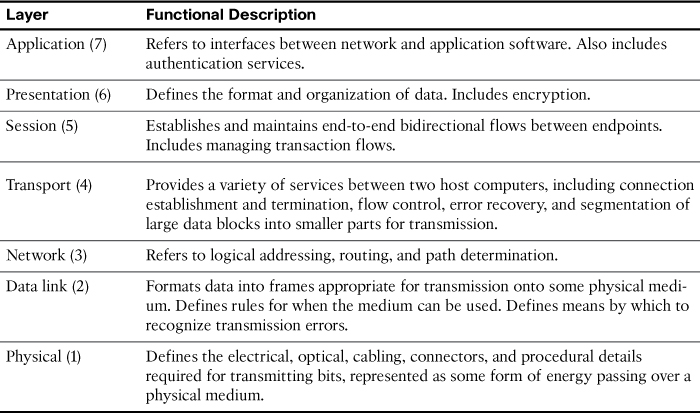
\includegraphics[scale=0.8]{OSI.jpg}
\end{center}
\vspace{2mm} %2mm vertical space
\noindent In this architecture, each layer serves the layer above it and, in turn, is served by the layer below it and control is passed from one layer to the next. If there are two parties to a communication session, data generated by each starts at the top layer, undergoing any required configuration and processing through the layers, and is finally delivered to the physical layer for transmission across the physical medium. \\ \par
\noindent In our case, most interfaces that are integrated on microcontrollers only cover the data link layer, with the physical layer being implemented externally. \\ \par
\newpage

\subsection{Implementations of OSI layers}
\subsubsection{Data link layer}
\noindent With reference to the OSI model, the UART in our project implements the data link layer (layer 2). \\ \par
\noindent In this layer, the data packets of ASCII characters consist of one start bit, 8 data bits, an even parity bit and one stop bits are transmitted with 9600 baud rate. \\ \par
\noindent The UART data link layer offer the even parity bit in terms of error checking. \\ \par
\subsubsection{Physical layer}
\noindent The full physical layer (layer 1) of the OSI in our case is implemented in the Spartan-3E FPGA Starter Kit using VHDL codes.\\ \par 
\noindent FPGA contains an array of programmable logic blocks, and a hierarchy of reconfigurable interconnects that allow the blocks
to be wired together. In most blocks, it includes the memory block. Therefore, the rest tasks in our project are processed in this layer. \\ \par  
\noindent The physical layer features include pulse shaper and serial communication. \\ \par  

\newpage
\chapter{Specifications}
In the sections below, there is a block diagram \ref{block diagram} of the design and a description of the block diagram with its modules \ref{diagram description}.\par 
\section{Block Diagram}\label{block diagram}
\begin{center}
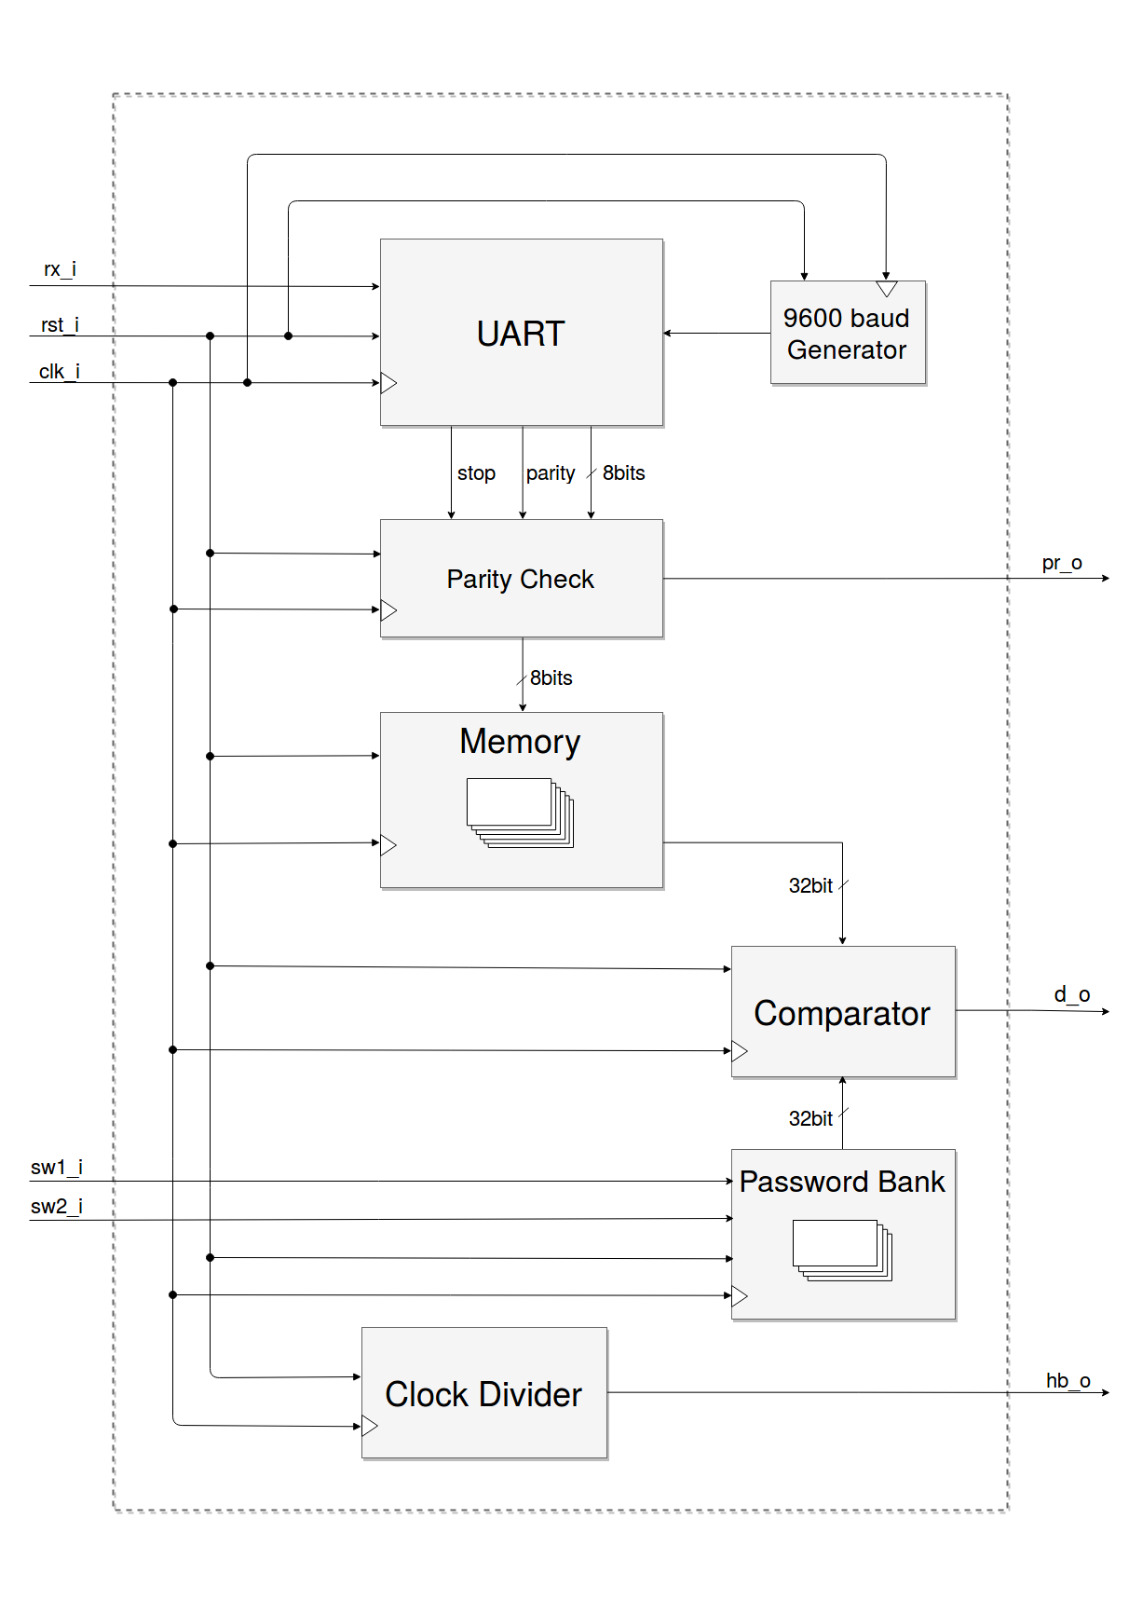
\includegraphics[scale=0.57]{block_diagram.png}
\end{center}
\newpage
\section{Diagram Description}\label{diagram description}In the diagram presented above in section \ref{block diagram}, there are five inputs and three outputs. All of the inputs are single bit inputs as well as the outputs. \\ \par
\noindent Two of the inputs are taken from switches on the board and their purpose is to select a pre-stored password. The reset input is taken from a push-button from the development board, as well as the clock signal which is taken from the board (50 MHz). The last input comes from a programmed micro-controller and brings the transmitted data into the ASIC. \\ \par
\noindent The outputs are realized on LEDs from the development board. There is an output which will signalize correct parity and another to signalize when the door opens. There is also an output which implements a heart-beat signal to show that the system is running. \\ \par

\noindent The ASIC should be able to input the data which is sent from the micro-controller. The UART receiving principal is implemented regarding this matter at 9600 baud rate line. After the data package is received, the device should check for correct parity. If the condition for correct parity is met, then the data bits from the package are stored in "memory". Finally, after the transmission of all characters is finished, the device should compare the transmitted characters with the switch-selected password (pre-stored characters). If there is a match, an LED should light up.  \\ \par

\noindent A brief description of each block/module inside the design is given below. \\ \par

\subsection{UART - Receiver}
\noindent This module gets an input from the micro-controller and the baud generator, as well as a clock and reset input. It receives a single bit data from the micro-controller at 9600 baud rate. However the sampling will not be done exactly on the rising or the falling edge of the transmitted bit, but roughly in the middle. The purpose of this is to improve the accuracy and reduce errors. After the stop bit, the module sends the received package of 8 bits data, parity bit and stop bit in the Parity Check module. \\ \par
\subsection{9600 Baud Generator}
\noindent This is the module which generates pulses for maintaining the 9600 baud rate transmission or in other words every 104.2 \si{\micro\second} a pulse is generated and send to the UART module. It works on the principle of dividing the clock of 50 \si{\mega\hertz} which is taken as an input.\\ \par
\subsection{Parity Check}
\noindent At this module the parity of the received package is checked. This is done because we want to check for possible errors in the transmission. For the purpose of this project, an even parity will be used, i.e. the number of logic-high bits in the data package (including the parity) should be even. If the parity is correct the 8 data bits are send to the memory , else and error occurred and the received package is dismissed.\\ \par
\subsection{Memory}
\noindent This module needs to store the characters which are received from the micro-controller. The memory stores characters that only passed the parity check. After the transmission, the characters are packed in a 32 bit vector and send to the Comparator module. The stored data is removed when a system reset is done.\\  \par
\subsection{Password Bank}
\noindent At this module, the device keeps the pre-stored characters/passwords. The characters encoding is ASCII. Each password can be selected by two switches which are the inputs of this module. The selected password is packed in a 32 bit vector and send to the Comparator module.\\ \par
\subsection{Comparator}
\noindent This is the module which receives packages of 32 bits from the Memory and from the Password Bank. Its duty is to check/compare both of those packages. If they have the same content, the Comparator sends an output which signalizes that the password is correct, i.e. the door opens. If the password is not correct the LED will not light up.\\  \par
\subsection{Clock Divider}
\noindent This module is used to create a pulse at a required frequency. It divides the system clock up to the particular frequency which should be generated. The pulse will be send as an output to an LED to implement a heart-beat signal on the board. The purpose of this heart-beat signal is to show that the system is running.\\  \par

\chapter{I/O Specifications}
All the I/Os which are used in the design are declared and specified here. It is also given a short description for each I/O as wall as the board pin which is used. \par
\vspace{5mm} %5mm vertical space

\section{Top-level}
\subsection{Inputs}
\begin{flushleft}
    \begin{tabular}{ | l | l | l | p{11cm} |}
    \hline
    Name & Bit(s) & Pin & Description \\ \hline
    rx\textunderscore i & 1 & R7 & This input brings the data which is sent from the micro-controller to the ASIC. \\ \hline
    clk\textunderscore i & 1 & C9 & This is the clock that is imported from the board which is used for realizing the design. The imported clock from the board is 50 MHz. \\ \hline
    rst\textunderscore i & 1 & N17 & This is the reset of the system. The purpose is to provide a reset state to all the working components. This signal is taken from a push-button on the board. \\ \hline
    sw1\textunderscore i & 1 & L14 & This is the input taken from switch number 1. The switch is located on the board where the design is realized. \\ \hline
    sw2\textunderscore i & 1 & H18 & This is the input taken from switch number 2. The switch is located on the board where the design is realized. \\ \hline
    \end{tabular}
\end{flushleft}

\subsection{Outputs}

\begin{flushleft}
    \begin{tabular}{ | l | l | l | p{11cm} |}
    \hline
    Name & Bit(s) & Pin & Description \\ \hline
    pas\textunderscore o & 1 & F12 & This is the output which will turn on/off an LED depending whether the door is open or closed. The LED is located on the board. \\ \hline
    l\textunderscore o & 1 & E11 & This output will set an LED on/off depending whether the parity is correct. The LED is located on the board. \\ \hline
    hb\textunderscore o & 1 & E12 & This output implements a heart-beat signal on an LED. \\ \hline
    \end{tabular}
\end{flushleft}

\newpage
\section{UART-Receiver}
\subsection{Inputs}
\begin{flushleft}
    \begin{tabular}{ | l | l | l | p{11cm} |}
    \hline
    Name & Bit(s) & Pin & Description \\ \hline
    rx\textunderscore i & 1 & R7 & This input brings the data which is sent from the micro-controller to the ASIC. \\ \hline
    clk\textunderscore i & 1 & C9 & This is the clock that is imported from the board which is used for realizing the design. The imported clock from the board is 50 MHz. \\ \hline
    rst\textunderscore i & 1 & N17 & This is the reset of the system. The purpose is to provide a reset state to all the working components. This signal is taken from a push-button on the board. \\ \hline
    bd\textunderscore i & 1 & / & This is the input taken from baud generator with shifted pulse for correct sampling. \\ \hline
    \end{tabular}
\end{flushleft}

\subsection{Outputs}

\begin{flushleft}
    \begin{tabular}{ | l | l | l | p{11cm} |}
    \hline
    Name & Bit(s) & Pin & Description \\ \hline
    l\textunderscore o & 1 & E11 & This output will set an LED on/off depending whether the parity is correct. The LED is located on the board. \\ \hline
    dat\textunderscore o & 8 & / & This is the output which contains the ASCII binary data. \\ \hline
    ena\textunderscore o & 1 & / & This output will send to enable baud generator. \\ \hline
    mem\textunderscore o & 1 & / & This output informs register when one password is received. \\ \hline
    par\textunderscore o & 1 & / & This output indicates the result of parity-check of the received package. \\ \hline
    cn\textunderscore o & 1 & / & This output announces the status of data input to password comparator. \\ \hline
    flg\textunderscore o & 1 & / &  \\ \hline
    s\textunderscore o & 1 & / & \\ \hline
    ss\textunderscore o & 2 & / &  \\ \hline
    
    \end{tabular}
\end{flushleft}

\vspace{2mm} %2mm vertical space
\section{Baud Generator}
\subsection{Inputs}
\begin{flushleft}
    \begin{tabular}{ | l | l | l | p{11cm} |}
    \hline
    Name & Bit(s) & Pin & Description \\ \hline
    clk\textunderscore i & 1 & C9 & This is the clock that is imported from the board which is used for realizing the design. The imported clock from the board is 50 MHz. \\ \hline
    rst\textunderscore i & 1 & N17 & This is the reset of the system. The purpose is to provide a reset state to all the working components. This signal is taken from a push-button on the board. \\ \hline
    ena\textunderscore i & 1 & / & This is the input taken from UART-Receiver which activates baud generator. \\ \hline
    \end{tabular}
\end{flushleft}

\subsection{Outputs}

\begin{flushleft}
    \begin{tabular}{ | l | l | l | p{11cm} |}
    \hline
    Name & Bit(s) & Pin & Description \\ \hline
    bd\textunderscore o & 1 & / & This is the onput which gives UART-Receiver shifted pulse for correct sampling. \\ \hline
    d\textunderscore o & 1 & / &  \\ \hline
    \end{tabular}
\end{flushleft}

\newpage
\section{Register}
\subsection{Inputs}
\begin{flushleft}
    \begin{tabular}{ | l | l | l | p{11cm} |}
    \hline
    Name & Bit(s) & Pin & Description \\ \hline
    clk\textunderscore i & 1 & C9 & This is the clock that is imported from the board which is used for realizing the design. The imported clock from the board is 50 MHz. \\ \hline
    rst\textunderscore i & 1 & N17 & This is the reset of the system. The purpose is to provide a reset state to all the working components. This signal is taken from a push-button on the board. \\ \hline
    par\textunderscore i & 1 & / & This input comes from UART-Receiver with the result of parity-check. \\ \hline
    mem\textunderscore i & 1 & / & This input contains information of whether one password is received from UART-Receiver. \\ \hline
    dat\textunderscore i & 8 & / & This is the input which contains the ASCII binary data from UART-Receiver. \\ \hline
    m\textunderscore i & 1 & / & This input taken from password comparator requests password. \\ \hline
    fs\textunderscore i & 1 & / &  \\ \hline
    
    \end{tabular}
\end{flushleft}

\subsection{Outputs}

\begin{flushleft}
    \begin{tabular}{ | l | l | l | p{11cm} |}
    \hline
    Name & Bit(s) & Pin & Description \\ \hline
    d\textunderscore o & 8 & / & This is the output which contains the ASCII binary data. \\ \hline
    g\textunderscore o & 1 & / &  \\ \hline
    \end{tabular}
\end{flushleft}

\vspace{2mm} %2mm vertical space
\section{Password Comparator}
\subsection{Inputs}
\begin{flushleft}
    \begin{tabular}{ | l | l | l | p{11cm} |}
    \hline
    Name & Bit(s) & Pin & Description \\ \hline
    clk\textunderscore i & 1 & C9 & This is the clock that is imported from the board which is used for realizing the design. The imported clock from the board is 50 MHz. \\ \hline
    rst\textunderscore i & 1 & N17 & This is the reset of the system. The purpose is to provide a reset state to all the working components. This signal is taken from a push-button on the board. \\ \hline
    dat\textunderscore i & 8 & / & This is the input which contains the ASCII binary data sent from Register. \\ \hline
    tno\textunderscore i & 1 & / & This input gets the status of data input from UART-Receiver. \\ \hline
    s1\textunderscore i & 1 & / & This is the input taken from switch number 1.  \\ \hline
    s2\textunderscore i & 1 & / & This is the input taken from switch number 2.  \\ \hline
    g\textunderscore i & 1 & / &  \\ \hline
    
    \end{tabular}
\end{flushleft}

\subsection{Outputs}

\begin{flushleft}
    \begin{tabular}{ | l | l | l | p{11cm} |}
    \hline
    Name & Bit(s) & Pin & Description \\ \hline
    m\textunderscore o & 1 & / & This output requests password after getting the switch value. \\ \hline
    p\textunderscore o & 1 & / &  This is the output which indicates whether the password is correct or not. \\ \hline
    \end{tabular}
\end{flushleft}


\newpage
\section{Heart-beat}
\subsection{Inputs}
\begin{flushleft}
    \begin{tabular}{ | l | l | l | p{11cm} |}
    \hline
    Name & Bit(s) & Pin & Description \\ \hline
    clk\textunderscore i & 1 & C9 & This is the clock that is imported from the board which is used for realizing the design. The imported clock from the board is 50 MHz. \\ \hline
    rst\textunderscore i & 1 & N17 & This is the reset of the system. The purpose is to provide a reset state to all the working components. This signal is taken from a push-button on the board. \\ \hline
    
    \end{tabular}
\end{flushleft}

\subsection{Outputs}

\begin{flushleft}
    \begin{tabular}{ | l | l | l | p{11cm} |}
    \hline
    Name & Bit(s) & Pin & Description \\ \hline
	hb\textunderscore o & 1 & E12 & This output implements a heart-beat signal on an LED. \\ \hline
    \end{tabular}
\end{flushleft}

% Here is the Bibliography of this document:
\begin{thebibliography}{1}

\bibitem{Rx}
\begin{flushleft}
Wikipedia - UART, \url{https://en.wikipedia.org/wiki/Universal_asynchronous_receiver-transmitter}
\end{flushleft} 

\bibitem{Fnc}
\begin{flushleft}
Wikipedia - Functional requirements, \url{https://en.wikipedia.org/wiki/Functional_requirement}
\end{flushleft}

\bibitem{OSI}
\begin{flushleft}
Wikibooks - Serial programming, \newline \url{https://upload.wikimedia.org/wikipedia/commons/1/1f/Serial_Programming.pdf}
\end{flushleft}

\bibitem{OSI}
\begin{flushleft}
ICND1 topic - OSI layers, \url{http://ptgmedia.pearsoncmg.com/imprint_downloads/informit/learninglabs/9780134213736/ch30.html}
\end{flushleft}

\bibitem{OSI}
\begin{flushleft}
Wikipedia - OSI model, \url{https://en.wikipedia.org/wiki/OSI_model}
\end{flushleft}

\bibitem{Prof}
\begin{flushleft}
Prof. Dr. -Ing. Andreas Sigelkow - Lecture Plan WS 2018/19
\end{flushleft}  
\end{thebibliography}


\end{document}